%**************************************************************************
%*
%*  Paper: ``INSTRUCTIONS FOR AUTHORS OF LATEX DOCUMENTS''
%*
%*  Publication: 2014 Winter Simulation Conference Author Kit
%*
%*  Filename: wsc14paper.tex
%*
%*  Date: January 31, 2001   Time:  9:45 PM
%*      BASE of current version: Feb 01, 2010 (primary WSC'10 LaTeX file)
%*
%*  Word Processing System: TeXnicCenter and MiKTeX
%*
%*
%*  All files need the following
\input{wsc14style.tex}     % download from author kit.  Style files for wsc formatting. Don't remove this line - required for generating the final paper!

\documentclass{wscpaperproc}
\usepackage{latexsym}
%\usepackage{caption}
\usepackage{graphicx}
\usepackage[tight,footnotesize]{subfigure}
\usepackage{mathptmx}

%
%****************************************************************************
% AUTHOR: You may want to use some of these packages. (Optional)
\usepackage{amsmath}
\usepackage{amsfonts}
\usepackage{amssymb}
\usepackage{amsbsy}
\usepackage{amsthm}
\usepackage{algorithm2e}
\usepackage{url}
%****************************************************************************



%
%****************************************************************************
% AUTHOR: If you do not wish to use hyperlinks, then just comment
% out the hyperref usepackage commands below.

%% This version of the command is used if you use pdflatex. In this case you
%% cannot use ps or eps files for graphics, but pdf, jpeg, png etc are fine.

\usepackage[pdftex,colorlinks=true,urlcolor=blue,citecolor=black,anchorcolor=black,linkcolor=black]{hyperref}

%% The next versions of the hyperref command are used if you adopt the
%% outdated latex-dvips-ps2pdf route in generating your pdf file. In
%% this case you can use ps or eps files for graphics, but not pdf, jpeg, png etc.
%% However, the final pdf file should embed all fonts required which means that you have to use file
%% formats which can embed fonts. Please note that the final PDF file will not be generated on your computer!
%% If you are using WinEdt or PCTeX, then use the following. If you are using
%% Y&Y TeX then replace "dvips" with "dvipsone"

%%\usepackage[dvips,colorlinks=true,urlcolor=blue,citecolor=black,%
%% anchorcolor=black,linkcolor=black]{hyperref}
%****************************************************************************



		



%
%****************************************************************************
%*
%* AUTHOR: YOUR CALL!  Document-specific macros can come here.
%*
%****************************************************************************

% If you use theoremes
\newtheoremstyle{wsc}% hnamei
{3pt}% hSpace abovei
{3pt}% hSpace belowi
{}% hBody fonti
{}% hIndent amounti1
{\bf}% hTheorem head fontbf
{}% hPunctuation after theorem headi
{.5em}% hSpace after theorem headi2
{}% hTheorem head spec (can be left empty, meaning `normal')i

\theoremstyle{wsc}
\newtheorem{theorem}{Theorem}
\renewcommand{\thetheorem}{ \arabic{theorem}}
\newtheorem{corollary}[theorem]{Corollary}
\renewcommand{\thecorollary}{\arabic{corollary}}
\newtheorem{definition}{Definition}
\renewcommand{\thedefinition}{\arabic{definition}}


%#########################################################
%*
%*  The Document.
%*
\begin{document}

%***************************************************************************
% AUTHOR: AUTHOR NAMES GO HERE
% FORMAT AUTHORS NAMES Like: Author1, Author2 and Author3 (last names)
%
%		You need to change the author listing below!
%               Please list ALL authors using last name only, separate by a comma except
%               for the last author, separate with "and"
%
%\WSCpagesetup{LastName1, LastName2, and LastNameLastAuthor}
\WSCpagesetup{Vasudevan, Bragard, Ventresque and Gregg}

% AUTHOR: Enter the title, all letters in upper case
\title{An evaluation of space partitioning methods and meta-heuristics based graph partitioning methods for partitioning road network simulations}

% AUTHOR: Enter the authors of the article, see end of the example document for further examples
% \author
% {
% 	\begin{figure*}[htb]
% 	{
% 		\centering
% 		\begin{tabular}{ccc}
% 		\phantom{Entries to adjust spacing - ignore} & \phantom{intermediate space} & \phantom{Entries to adjust spacing - ignore} \\
% 		Aravind Vasudevan & & Quentin Bragard \\
% 		David Gregg & & Anthony Ventresque \\
% 		\\
% 		Trinity College Dublin & & University College Dublin \\
% 		Dublin, Ireland & & Dublin, Ireland
% 		\end{tabular}
% 		\caption{Example title page heading with 2 authors from different institutions.\label{fig: 2 different}}
% 	}
% 	\end{figure*}
% }
\author{Aravind Vasudevan\textsuperscript{1}, Quentin Bragard\textsuperscript{2}, Anthony Ventresque\textsuperscript{2} and David Gregg\textsuperscript{1}\\ [12pt]
\textsuperscript{1} School of Computer Science and Statistics, Trinity College Dublin\\
\textsuperscript{2} Computer Science Department, University College Dublin\\
}
% \author{Aravind Vasudevan\\ [12pt]
% School of Computer Science and Statistics\\
% Trinity College Dublin\\
% \and
% Quentin Bragard\\ [12pt]
% Computer Science Department\\
% University College Dublin\\
% \and
% Anthony Ventresque\\ [12pt]
% Computer Science Department\\
% University College dublin\\
% \and
% David Gregg\\ [12pt]
% School of Computer Science and Statistics\\
% Trinity College Dublin
% }
%\author{Aravind Vasudevan\\ [12pt]
% \author{Aravind Vasudevan\\ 
% David Gregg\\ [12pt]
% School of Computer Science and Statistics\\
% Trinity College Dublin\\
% \and
% Quentin Bragard\\ 
% Anthony Ventresque\\ [12pt]
% Computer Science Department\\
% University College Dublin\\
% }
% \author{Andreas Tolk\\ [12pt]
% SimIS Inc.\\
% 200 High St. \#305\\
% Portsmouth, VA 23704, USA\\
% % Multiple authors are entered as follows.
% % You may also need to adjust the titlevbox size in the preamble - search for titlevboxsize
% \and
% Saikou Diallo \\[12pt]
% Virginia Modeling Analysis \& Simulation Center \\
% Old Dominion University\\
% 1030 University Boulevard\\
% Suffolk, VA 23435, USA \\
% \and
% Ilya O. Ryzhov\\ [12pt]
% Robert H. Smith School of Business\\
% University of Maryland\\
% 4322 Van Munching Hall\\
% College Park, MD 20742, USA\\
% \and
% Levent Yilmaz\\ [12pt]
% Computer Science and Software Engineering\\
% Auburn University\\
% 3116 Shelby Center\\
% Auburn, AL 36849, USA
% }

\maketitle

\section*{ABSTRACT}
Abstract goes here.  

\section{MOTIVATION}

Introduction goes here.

Our \textbf{key contributions} in this paper are:

\begin{itemize}
\item 
\item 
\item 
\item 
\end{itemize}

The rest of the paper is arranged as
follows. 

\section{RELATED WORK}
\label{sec:rela}
\section{FORMALIZATION OF THE PROBLEM STATEMENT}
\label{sec:form}

In this paper we conduct a statistically significant comparison of different methods of partitioning a road network graph based on some metrics. This section defines what a road network graph is and presents the formal definition of the metrics in the context of this formal descriptions.

\subsection{The Road Network Graph}
\label{sec:form-road-netw-grap}
The road network of a city can be represented by a directed cyclic graph~\cite{holden1995mathematical} $G(V, E)$ where $V$ denotes the vertex set and $E$ denotes the edge set. Every edge $e_{ij} \in E$ in the graph represents a unidirectional road in the city that connects intersection $v_i$ to intersection $v_j$. Every vertex $v_i \in V$ denotes an intersection of two or more roads. A weight $w_{ij}$ is associated with the edge $e_{ij}$ that is representative of the traffic that flows through that road. As discussed in Section~\ref{sec:futu}, we plan on increasing the number of weights that can be associated with every edge to be able to represent the number of lanes, length of the road, importance of the road etc.

\subsection{Partitioning a graph}
\label{sec:form-part}
For the sake of completeness of the graph definition, we also assign weights to the vertices denoted by $W_i$, which is defined as follows :
\begin{equation}
\label{eq:vertex-weight}
W_i = \sum\limits_{\forall j \in neighbours(i)} w_{ij}
\end{equation}

where $neighbours(i)$ is the set of all nodes in $V$ that receive an outgoing edge from $v_i$.


\subsection{Formalizing the objective function}
\label{sec:form-obje-func}

We define a partitioning scheme, $\zeta$ as 

% The total application latency in a parallel setting is the addition of
% the computation time and the communication
% time~\cite{ssan05,ajai04}. Given some application node $i \in V_t$
% mapped to some resource $j \in V_r$. The latency for that node is
% computed as: $((w^t_1(i)/W^r_1(j)\times w^t_0(i))/W^r_0(c))+
% (w^e(e)/W^c(c)) | e = (i,k), k \neq i, \forall k \in V_t, c = (j,l), l
% \neq j, \forall l \in V_r $. In this formulation for some given
% task graph node $i$, we first calculate the number of vectorized
% instructions that need to be performed (by diving the required vector
% length with the vector capacity of the resource node), this gives us the
% total number of vector instructions that would be performed on the
% resource node $j$. Next, we multiply the number of vector instructions
% to be performed by the number of iterative (non-vectorized) instructions
% required, this in turn gives us the total number of instructions to be
% performed by that task graph node. Finally, we find the computation
% latency by dividing this total number of instructions with the MIPS
% value of the resource vertex. For communication on the other hand, we
% calculate the communication latency, by dividing the number of required
% bits to be transferred by the bandwidth of the resource.

% Given the task graph and the resource-graph, let $\zeta$ be all possible
% mappings of the application on the resource-graph. For a particular
% mapping $\mathcal{M}$ defined as $\zeta_\mathcal{M}$ on some resource $s
% \in V_r$ the mapping latency is defined as:

% \begin{equation

%   \begin{array}{c}
%     Latency^{\zeta_\mathcal{M}}_s = \\
%     \\
%     \sum_{\forall i \in V_t \wedge
%       \zeta_\mathcal{M} = s} ((w^t_1(i)/W^r_1(s)\times w^t_0(i))/W^r_0(c))
%     \\
%     +
%     \\
%     \sum_{\forall i \in V_t \wedge
%       \zeta_\mathcal{M} = s} w^e(e) / W^c(c)\\ 
%     s.t., e = (i,k), k \neq i, \forall k
%     \in V_t \wedge\  c = (s,l), l \neq s, \forall l \in V_r
%   \end{array}
%   \label{eq:1}
% \end{equation}

% Finally, the complete application latency can then be defined as: 
% \begin{equation}
%   \tag{OBJECTIVE\_FUNCTION}
%   \label{eq:2}
%   Latency^{\zeta_\mathcal{M}} = max_{s}
%   ({Latency^{\zeta_\mathcal{M}}_s}), \forall s \in V_t
% \end{equation}

The objective of our framework is to minimize the total application
latency as described in Equation~(\ref{eq:2}).
\section{META HEURISTICS BASED GRAPH PARTITIONING ALGORITHMS}
\label{sec:meta}

\subsection{Simulated Annealing}
\label{sec:simu-anne}

\begin{scriptsize}
\begin{algorithm}[ht!]
  % \vspace{-.9cm}
  \smaller{
    \caption{The Simulated Annealing Algorithm}
    \label{algo:SA}
    % \DontPrintSemicolon
    \KwIn{Initial Mapping $\lambda_0$ and Starting and Final Temperatures
$\mathcal{T}_0$, $\mathcal{T}_f$}
    \KwOut{Best Mapping $\lambda_{best}$}
    $\lambda_{current} \leftarrow \lambda_0$ \;
    $C_{current} \leftarrow objective\_function(\lambda_0)$;  //calculate initial objective function value\;
    $\lambda_{best} \leftarrow \lambda_{current}$\;
    $C_{best} \leftarrow C_{current}$\;
    \For {$i \leftarrow 0\ to\ \infty$}{
      $\mathcal{T}_{current} \leftarrow next\_temperature(\mathcal{T}_0,i)$\;
      $\lambda_{new} \leftarrow move(\lambda_{current}, \mathcal{T})$\;
      $C_{new} \leftarrow objective\_function(\lambda_{new})$\;
      $\Delta C \leftarrow C_{new} - C_{current}$\;
      $p \leftarrow acceptance\_probability(\Delta C, \mathcal{T}_{current})$\;
      \If{$\Delta C < 0$ or $r < p$}{
        \If{$C_{new} < C_{best}$}{
          $\lambda_{best} \leftarrow \lambda_{new}$;\ $C_{best} \leftarrow
          C_{new}$;\ 
          $\lambda_{current} \leftarrow \lambda_{new}$;\ $C_{current} \leftarrow C_{new}$\;
        }
      }
      \Else{
        \If{$\mathcal{T}_{current} \leq \mathcal{T}_f \| executionTime \geq maxTime$}{break}
      }
    }
    \Return $\lambda_{best}$
  }
\end{algorithm}
\end{scriptsize}

Simulated Annealing~\cite{kirkpatrick1983optimization} is an adaptation of the Metropolis-Hastings algorithm for solving the problem of locating a good approximation of the global optimum of a given
function, $\mathcal{F}: \mathbb{R} \rightarrow \mathbb{R}$, which has a
large search space. This large number of states, as discussed in Section~\ref{sec:form-part}, makes exhaustive enumeration to find optimal solutions, not feasible.

SA is a heuristic algorithm that explores the search space by inspecting one valid state at each iteration. Each of these inspected states are evaluated by an ``objective function'' which tells us how ``good'' or ``bad'' this state is. The ``goodness'' in an SA algorithm is problem dependent and in our case it is given by the metrics defined in Section~\ref{sec:form-obje-func}. The algorithm progresses by inspecting a candidate state at each iteration and it either accepts it as its current state or discards the state and ``moves'' on to another state. We define a move as the generation of the next candidate states and this progress is governed by a global time-varying parameter called the ``temperature'' which changes based on an ``annealing schedule''.

The algorithm always accepts a move to a better solution, i.e. a new state which has a ``better'' objective function value than the current state. When this value is worse however, the SA algorithm accepts this move with a certain ``acceptance probability'', that changes with the current temperature. When the temperature is high, the algorithm accepts moves to a worse solution with a higher probability; as the temperature reduces over time, this probability decreases as well.

 Every Simulated Annealing method is characterized by the definition of its core functions and parameters. One such core function is the ``move'' function which defines how the next candidate state is generated. We formally define a this function as,

\begin{equation}
\label{eq:move-func}
move(\lambda_G, \mathcal{T}) =  \lambda_G^{'}
\end{equation}

\noindent where $\lambda_G^{'}$ is a new partitioning scheme which also maps each intersection to exactly one partition. The move function takes as input the current partitioning scheme $\lambda_G$ and the current temperature and describes how the generation of $\lambda_G^{'}$ is done. In this paper we present a few variations of the SA algorithm, in terms of the ``move'' as follows.

\subsubsection{Standard Move}
\label{sec:opti-std}
Conventional wisdom suggests that all move functions should be random 

\subsubsection{Global Edge Labelling}
\label{sec:opti-glob-edge}

\subsubsection{Local Edge Labelling}
\label{sec:opti-loca-edge}

\subsection{Genetic Algorithm}
\label{sec:gen-algo}

\begin{scriptsize}
\begin{algorithm}[ht!]
  % \vspace{-.9cm}
  \smaller{
    \caption{The Genetic Algorithm}
    \label{algo:ga}
    % \DontPrintSemicolon
    %\KwIn{Initial Mapping $\lambda_0$ and Starting and Final Temperatures $\mathcal{T}_0$, $\mathcal{T}_f$}
    %\KwOut{Best Mapping $\lambda_{best}$}
    Choose an initial random population of individuals\\
    Evaluate the fitness of the individuals\\
    \While{Termination criteria not met}{
      Select the \textit{best} ``n'' individuals to be used by the genetic operators\\
      Generate new offsprings by using the genetic operators\\
      Evaluate the objective function value for these offsprings\\
      Replace the \textit{worst} ``k'' individuals of the current population with the best ``k'' individuals from the offsprings\\
    }
  }
\end{algorithm}
\end{scriptsize}

Genetic Algorithm is a heuristic search\{cite core paper\} algorithm that mimics the natural selection process. This heuristic algorithm is often used\{cite usage in general context\} for solving optimization problems with large search spaces and it belongs to a larger class called Evolutionary Algorithms.

In the context of the problem at hand, we follow the definition for the search space from Section~\ref{sec:form-part}, as a 2-dimensional space with one axis representing the intersections and the other the partition IDs. Hence each point in the space becomes a \textit{\{intersection,partition\}} pair.

\noindent To characterize a genetic algorithm, we require two things :
\begin{itemize}
	\item A \textbf{genetic representation} of the solution space as shown in Figure~\ref{fig:gene-repr}
	\item An \textbf{objective function} to evaluate solutions as discussed in Equation~\ref{eq:obje-func} from Section~\ref{sec:form-obje-func}
\end{itemize}

Once this is fixed, we initialize the algorithm by generating a set of random solution vectors and assigning that as the initial population. The initial population size is problem specific and in our case it is 400 which is sufficiently a large sample and small enough to ensure fast generation of offsprings. We have chosen to generate the initial population randomly as opposed to generating it with some seed, to cover a wider range of candidates from our large search space. We then apply a set of genetic operators as discussed in Section~\ref{sec:gene-oper} to generate the next population. This process is repeated and the ``n'' best solutions are retained at every step. We terminate the algorithm once a fixed time has passed by. Algorithm~\ref{algo:ga} gives an algorithmic overview of the above mentioned process.

\subsubsection{Genetic Operators}
\label{sec:gene-oper}
Although there are a lot of genetic operators to choose from\{cite core paper and some new papers\}, we employ the \textbf{mutation} and \textbf{crossover} operators for the purpose of this comparison
\begin{itemize}
	\item \textbf{mutation} - 
	\item \textbf{crossover} - 
\end{itemize}
\section{EXPERIMENTS AND RESULTS}
\label{sec:exps}

% We show the speedup obtained using our improved heuristics against the
% conventional heuristics for SA as prescribed by~\cite{hors06}. We also
% compare the results we obtain against the K-way graph partitioning
% algorithm~\cite{gkar95} and heterogeneous bin packing
% heuristic~\cite{mmar11}.

% \subsection{K-way graph partitioning}
% \label{sec:k-way-graph}

% Graph partitioning plays an important role in the multi-processor and
% VLIW scheduling and partitioning
% algorithms~\cite{aale01,kpur99,enys98}. K-way graph partitioning is an
% important algorithm, which partitions a given graph into K or less
% parts, resulting in load balanced allocations. K-way partitioning mixed
% with min-edge cuts can form a good tool to partition a task-graph onto a
% multi-processor system, resulting in equal utilization of PEs and
% reduced communication costs. We have utilized the Metis~\cite{gkar95}
% graph partitioning tool to perform a K-way graph partitioning onto
% heterogeneous multi-processor architectures for comparison purposes.

% Metis is a graph partitioner, which implements K-way partitioning with
% min-edge cut as the primary objective. The weights on the graph nodes
% are represented as constraints. Each graph node can have multiple-node
% weights representing different criteria. The edges between nodes can be
% weighted themselves, but as opposed to nodes, edges can only be
% decorated with a single weight. Moreover, in Metis one can use a concept
% called ``tp-weights'', which give preference to different node
% constraints when performing load-balancing during K-way graph
% partitioning~\cite{gkar95}. % These are the only features of Metis
% % that we required when implementing our algorithm. Metis provides a
% % number of other features, which the readers can lookup
% % in~\cite{gkar95}.

% The gist of our K-way task partitioning approach onto a heterogeneous
% multi-core architecture is as follows:

% \begin{itemize}

% \item Our resource graph is first described as a simple graph in
%   Metis. In this description each of the two capabilities $W^i_0$ and
%   $W^i_1$ are described as two constraints for each node in the
%   graph. The communication bandwidth is described as edge weights in
%   Metis.

% \item Once we have the resource graph in the Metis format we calculate
%   the tp-weights. There are two tp-weights generated, one for each of
%   the resource node capabilities. Let us revisit the 4 $\times$ 4 mesh
%   shown in Figure~\ref{fig:1r}. For each processor the MIPS tp-weight is
%   calculated by the formula: $W^i_0/\sum_{\forall i \in
%     V_r}(W^i_0)$. Similarly, we can easily calculate the tp-weight
%   metric for each PEs vector length capability as: $W^i_1/\sum_{\forall
%     i \in V_r}(W^i_1)$. These fractions give a relative approximation of
%   the capabilities of each PE compared to the other. For example, given
%   two nodes with $W^0_0 = 100$ and $W^1_0 = 50$, then the tp-weights for
%   the first node has a tp-weight of, $0.667$, while the second has a
%   tp-weight of, $0.333$.

% \item The nodes in our task graph are described as graph nodes in the
%   Metis format. The two requirements ($R^i_0$ and $R^i_1$) for each task
%   node are described as two constraints in the Metis node format. The
%   edge weights in our task graph are described as edge weights in the
%   Metis graph format.

% \item Once we have the task graph described in the Metis format along
%   with the tp-weight metric for each PE in the resource graph. We ask
%   for a $|V_r|$ partition from Metis, giving the tp-weight metric for
%   each constraint of the task graph.

% \item The resultant partition is then used to calculate the objective in
%   Equation~(\ref{eq:2}).

% \end{itemize}

% \subsection{Heterogeneous bin packing heuristic}
% \label{sec:heter-bin-pack}

% Heuristic bin packing solutions have given good results in the general
% case~\cite{ecof78}. Comparing with the heterogeneous bin packing
% heuristic~\cite{mmar11} allows us to gauge the effectiveness of our
% algorithm against a standard technique.

% Let $\mathcal{I}$ be the items to be accommodated into the bins and let
% $\mathcal{K}$ be the set of bins available.  From the standpoint of the
% mapping problem, $\mathcal{I}$ refers to the set of task graph nodes
% ($|V_t|$) and $\mathcal{K}$ refers to the nodes in the resource graph
% ($|V_r|$). Similar to the Knapsack problem~\cite{sski08}, by which A-BFD
% (\textit{Adaptive Best First Decreasing}) is inspired, each element $i
% \in \mathcal{I},\ \mathcal{K}$ has two constraints on them represented
% by $c_i$ (cost), which translates to the PE capability $W^i_0$ and $V_i$
% (volume), which translates to the capability $W^i_1$, respectively.
% % Right off the bat, this seems to be a significant advantage, our
% % framework has over heterogeneous bin packing, as \textit{A-BFD} only
% % works with two constraints whereas our framework poses no such
% % restrictions.
% \textit{A-BFD} proceeds to sort $\mathcal{I}$ according
% to non-increasing order of their volume and sorts $\mathcal{K}$
% according to non-increasing order of the ratio $c_i/V_i$. Then, it
% proceeds to allocate items from $\mathcal{I}$ into best bins $b \in
% \mathcal{S}$. A ``best" bin, i.e., the bin with maximum free space, is
% defined as the bin volume minus the sum of volumes of the items loaded
% into it. % In the mapping problem setting, this becomes a double edged
% % sword as it boils down to a single constraint solving problem giving
% % higher priority to the second constraint (vector requirement of the
% % application-tasks $w^t_1(i)$ and vector capability of the resources
% % $W^r_1(i)$).

% The post pass in \textit{A-BFD} chooses every bin that has at least one
% item allocated to it and tries to find an empty bin, that has a higher
% or equal volume than the allocated volume on the chosen bin but also has
% a lower cost. If it finds such an empty bin, then it transfers all the
% items allocated to the chosen bin to the newly found empty bin which is
% cheaper. One of the main advantages of \textit{A-BFD} is that it is very
% fast with a best case complexity of $O(N_\mathcal{I})$ without the post
% pass, where $N_\mathcal{I}$ is the number of items (number of tasks
% $|V_t|$ in the application graph $G_t$). Including the post pass, the
% best case complexity becomes $O(N_\mathcal{I} + N_\mathcal{K})$ where
% $N_\mathcal{K}$ is the number of bins (number of PEs $|V_R|$ in the
% resource graph $G_r$).

% \subsection{The experimental setup}
% \label{sec:experimental-setup}

% We need to setup the resource graph and the task graph for experimental
% purposes. Here, we describe our setup for both.

% \subsubsection{The resource graph setup}
% \label{sec:resource-graph-setup}

% The experimental section consist of the following:

% \begin{enumerate}

% \item An multi-core system with \numtplgynodes nodes. A node could be
%   just a multi-core CPU or a multi-core CPU with a GPU attached to
%   it. \numtplgynodes varies in a normal distribution from 2 to 32.

% \item The bandwidth is selected from a set \mbox{$\bwset = \{B_1, B_2, ...,
%   B_{|\bwset|}\}$}. Every communication link weight ($W^c$) is selected
% from the set \bwset. The elements of the set \bwset varies in the normal
% distribution: 10Mb/s to 1Gb/s, representative of the multi-core
% connection networks in today's machines.

% \item A set of \gpunum GPUs where \gpunum is at most \numtplgynodes. The
%   GPUs are connected in the network at pre-determined locations, chosen
%   randomly in the normal distribution of 25\% to 75\% of $|V_r|$.

% \item A set $\veclenset = \{V_1, V_2, V_3, ... V_{|\veclenset|}\}$ where
%   $V_i$ is a power of 2.  Every GPU in this experiment has a vector
%   length of $V_i$ where $V_i$ is sampled randomly from the set
%   \veclenset. The elements of set \veclenset are chosen from a normal
%   distribution ranging from 1024 to 16284.

% \item A set $\corenumset = \{C_1, C_2, C_3, ... C_{|\corenumset|}\}$
%   where $C_i$ is a power of 2.  Every CPU in this experiment has $C_i$
%   cores where $C_i$ is sampled randomly from the set \corenumset.

% \item A set $\mipsset = \{M_1, M_2, M_3, ... M_{|\mipsset|}\}$ where
%   $M_i$ is a power of 2.  Every $C_i \in \corenumset$ and GPU in this
%   experiment has a MIPS count of $M_i$ where $M_i$ is sampled randomly
%   from the set \mipsset. The elements of set \mipsset are chosen from a
%   normal distribution ranging from 100 to 1000000.

% \end{enumerate}

% For given values of \numtplgynodes, \gpunum, \veclenset, \corenumset,
% and \mipsset and a given application, let the $k$-th \ul{trial} be
% defined as one execution of the following sequence of steps.

% \begin{itemize}

% \item For each GPU $G_i$, sample \veclenset and \mipsset randomly to
%   determine its vector length $V_i$ and MIPS count $M_i$. \label{i1}

% \item For each CPU $P_i$, sample \corenumset randomly to determine the
%   number of cores $C_i$ in the processor $P_i$.~\label{i2}

% \item For each core $C_i$ in the processor $P_i$ sample $V_i$ and $M_i$
%   randomly from set \veclenset and \mipsset.

% \item Use our framework to extract data and task parallelism that is
%   best utilizable by the heterogeneity created by parameters in items 1,
%   2, and 3 above. Determine the execution time
%   $Latency^{\zeta_\mathcal{M}}$.

% \end{itemize}

% An experiment, \expt(\numtplgynodes, \gpunum, \veclenset, \corenumset
% \mipsset), consists of conducting enough of the above trials so that
% width of the 95\% confidence interval on the average value of
% $Latency^{\zeta_\mathcal{M}}$ is less than 10\% of the average
% value. This results in a variable number of trials with different
% experimental setups. Note that two trials differ from each other only in
% the seed for the random number generator.  This reduces the dependence
% of our results on a lucky sequence of numbers from the random number
% generator.

% \subsubsection{The task graph setup}
% \label{sec:task-graph-setup}

% We chose 5 applications: binomial option pricing (a financial
% derivatives application), 2-dimensional convolution (for image
% processing), gram Schmidt linear algebra kernel, 2-dimensional
% Gauss-Seidel stencil computations, and finally our motivating example
% itself the 2-dimensional Jacobi stencil computation. Next for these 5
% applications, we varied the vector strip from 10 to 50, which resulted
% in graphs varying from around 50 to 5000 nodes and with 23 to 12,000
% edges. For example, given a task node with a vector length requirement
% ($w^i_1$) of 30,000 elements, a vector strip of 10 means dividing the
% total vector requirement by 10, which results in 10 nodes each requiring
% 3000 vector elements. Similarly, the instruction count ($w^i_0$) for
% each node varies depending upon the application at hand.

% A detailed description of the applications and their features is shown
% in Table~\ref{tab:1}. In general the vector requirement of the
% applications in our benchmark suite varies from 1000 to 1 Million
% elements. The instruction count varies from around 1 to 0.3 billion. The
% edge weights depicting the amount of data transfer on the other hand
% varies from 3000 bytes to almost 4.8 Mega byte.

% \begin{table}[h!]
%   \centering
%   \begin{tabular}{|c|c|c|c|}
%     \hline
%     \textbf{Application} & \textbf{Vector strip} & $|V_t|$ & $|E_t|$ \\
%     \hline
%     \multirow{5}{*}{Binomial option pricing} & 10 & 82 & 206 \\
%     & 20 & 102 & 306 \\
%     & 30 & 122 & 406 \\
%     & 40 & 142 & 506 \\
%     & 50 & 162 & 606 \\
%     \hline
%     \multirow{5}{*}{Convolution} & 10 & 79 & 143 \\
%     & 20 & 89 & 173 \\
%     & 30 & 99 & 203 \\
%     & 40 & 109 & 233 \\
%     & 50 & 119 & 263 \\
%     \hline
%     \multirow{5}{*}{Gram Schmidt} & 10 & 228 & 443 \\
%     & 20 & 838 & 1653 \\
%     & 30 & 1848 & 3663 \\
%     & 40 & 3258 & 6473 \\
%     & 50 & 5068 & 10083\\
%     \hline
%     \multirow{5}{*}{Gauss-Seidel} & 10 & 227 & 531 \\
%     & 20 & 837 & 2041 \\
%     & 30 & 1847 & 4551 \\
%     & 40 & 3257 & 8061 \\
%     & 50 & 5067 & 12571\\
%     \hline
%     \multirow{5}{*}{Jacobi} & 10 & 48 & 130 \\
%     & 20 & 78 & 240 \\
%     & 30 & 108 & 350 \\
%     & 40 & 138 & 460 \\
%     & 50 & 168 & 570\\
%     \hline
%   \end{tabular}
%   \caption{The task graph setup}
%   \label{tab:1}
% \end{table}

% \subsection{Experimental results}
% \label{sec:results}

% The comparison of our simulated annealing approach with other techniques
% are described in the next sub sections. In all the upcoming comparisons
% we set the value of $q=0.75$ in our SA and standard SA techniques. This
% value of $q$ is a good compromise between a slow running SA heuristic vs
% application latencies, since a bigger value of $q$, results in larger
% explored state space. For the aforementioned experimental setup our and
% standard SA techniques were run for 10 minutes.

% \subsubsection{Comparison with K-way partitioning}
% \label{sec:comparison-with-k}

% The results comparing K-way graph partitioning with our SA heuristic is
% shown in Figure~\ref{fig:metis}. The 3D surface graphs shown in
% Figure~\ref{fig:metis} consist of two surfaces. Each surface plots the
% execution latency of the application, in $log_{10}(sec)$ scale, on the
% Z-axis. The X and Y axes show the number of PEs in the underlying
% architecture and the vector strip sizes, respectively.

% The surface produced by the K-way partitioning heuristic is above the
% surface created by our SA heuristic for most applications, other than
% convolution and Jacobi. The major statistics comparing the two
% approaches is provided in Table~\ref{tab:2}. In Table~\ref{tab:2}, The
% \textbf{Max latency} and the \textbf{Min latency} columns, provide the
% maximum and minimum application latencies observed in
% Figure~\ref{fig:metis} for each of the applications. The last column
% gives the \% of points in the surfaces that were better in our SA
% technique compared to K-way graph partitioning.

% \begin{figure*}[t!]
%   \centering
%   \subfigure[Binomial Option Pricing]{
%     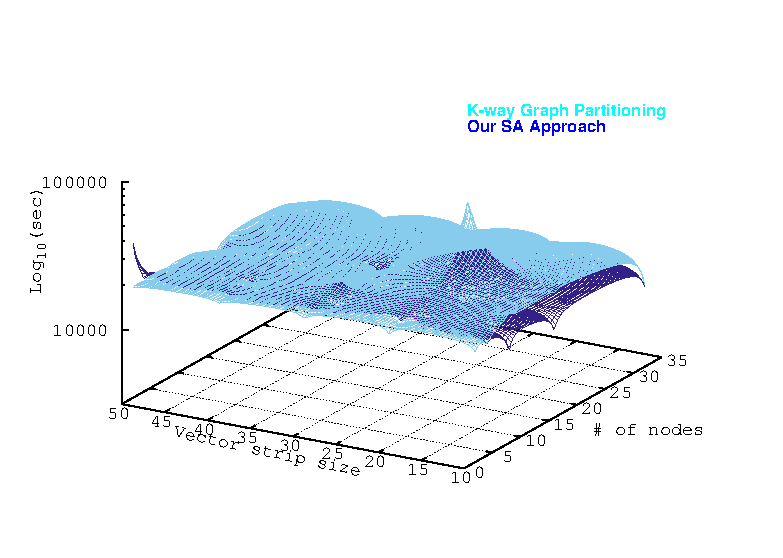
\includegraphics[angle=0, scale=0.6]{./figures/bin_metis_surface}
%     \label{fig:bin1metis}
%   }
%   \subfigure[2 Dimensional Convolution]{
%     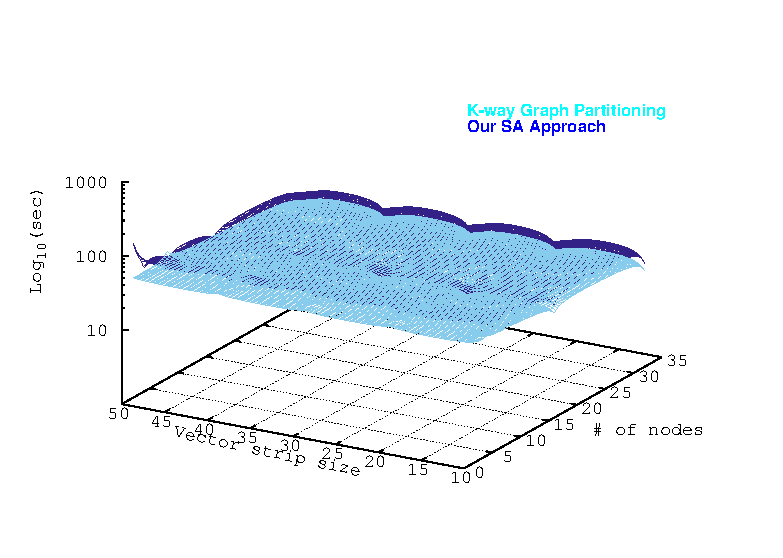
\includegraphics[angle=0, scale=0.6]{./figures/conv_metis_surface}
%     \label{fig:conv1metis}
%   }
%   \subfigure[Gram Schmidt linear-algebra kernel]{
%     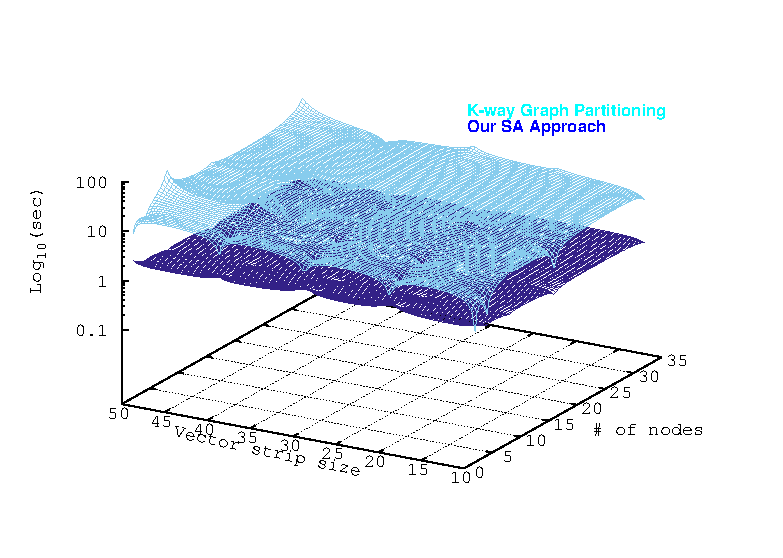
\includegraphics[angle=0, scale=0.6]{./figures/gram_metis_surface}
%     \label{fig:gram1metis}
%   }
%   \subfigure[2 Dimensional Seidel stencil computation]{
%     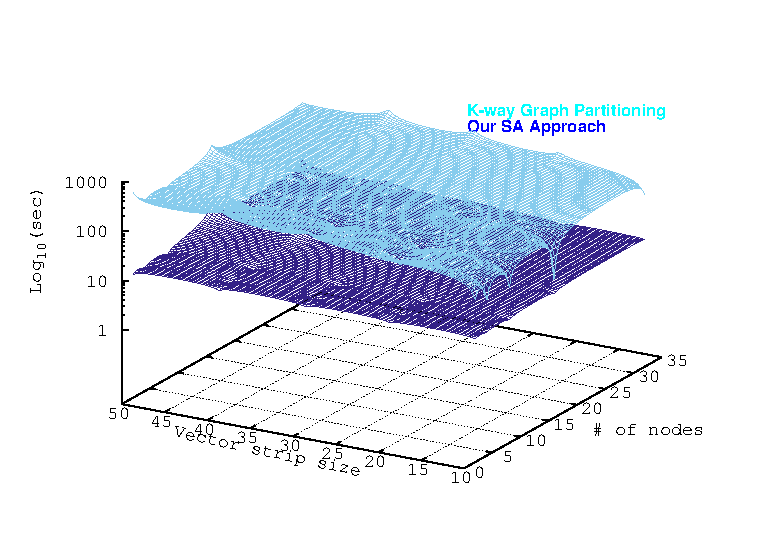
\includegraphics[angle=0, scale=0.6]{./figures/sei_metis_surface}
%     \label{fig:sei1metis}
%   }
%   \subfigure[2 Dimensional Jacobi stencil computation]{
%     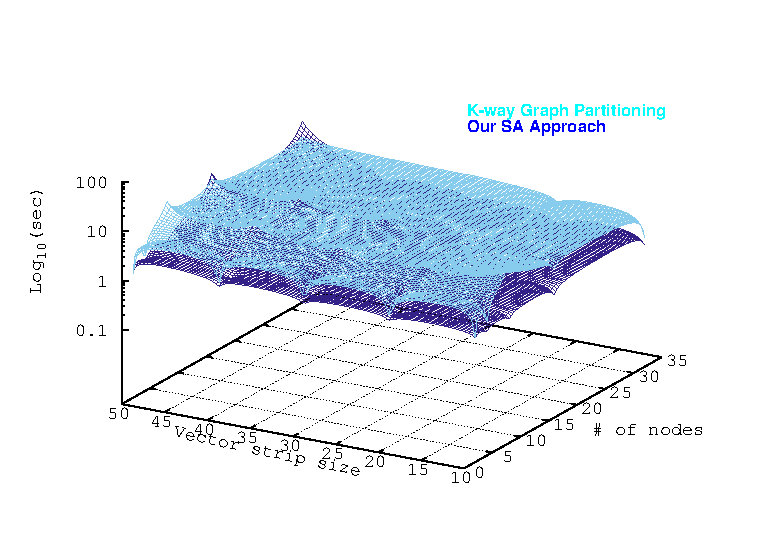
\includegraphics[angle=0, scale=0.6]{./figures/jac_metis_surface}
%     \label{fig:jacl1metis}
%   }
%   \caption{Comparison of application latencies: Our SA approach Vs K-way
%   graph partitioning (looks better in color)}
%   \label{fig:metis}
% \end{figure*}

% \begin{figure*}[t!]
%   \centering \subfigure[Major statistics comparing K-way graph
%   partitioning and our SA approach for Figure~\ref{fig:metis}]{
%     % \begin{table*}[t!]
%       \centering
%       \begin{tabular}{|c|c|c|c|c|c|}
%         \hline
%         \textbf{Application} &
%         \multicolumn{2}{|c|}{\textbf{Max latency (sec)}} &
%         \multicolumn{2}{|c|}{\textbf{Min latency (sec)}} &
%         \textbf{Our SA better than K-way (\%)} \\
%         \hline
%         & {K-way} & {Our SA approach} &
%         {K-way} & {Our SA approach} & K-way vs Our SA approach\\
%         \hline
%         Binomial option pricing & 79947.2 & 53404.8 & 11218.1 & 10975.5 & 94 \\
%         \hline
%         Convolution & 52.85 & 124.309 & 19.64 & 19.64 & 12\\
%         \hline
%         Gram Schmidt & 54.13 & 2.96 & 1.33 & 0.91 & 64\\
%         \hline
%         Gauss-Seidel & 542.44 & 32.99 & 9.67 & 9.67 & 68\\
%         \hline
%         Jacobi & 16 & 14.69 & 0.95 & 0.89 & 32\\
%         \hline
%       \end{tabular}
%       % \caption{Major statistics comparing K-way graph partitioning and our
%       %   SA approach}
%       \label{tab:2}
%     % \end{table*}
%   }
%   \subfigure[Major statistics comparing heterogeneous bin packing and our
%       SA approach for Figure~\ref{fig:ho}]{
%     % \begin{table*}[t!]
%     \centering
%     \begin{tabular}{|c|c|c|c|c|c|}
%       \hline
%       \textbf{Application} &
%       \multicolumn{2}{|c|}{\textbf{Max latency (sec)}} &
%       \multicolumn{2}{|c|}{\textbf{Min latency (sec)}} &
%       \textbf{Our SA better than HBP (\%)} \\
%       \hline
%       & {HBP} & {Our SA approach} &
%       {HBP} & {Our SA approach} & HBP vs Our SA approach\\
%       \hline
%       Convolution & 215741 & 124.309 & 98.45 & 19.64 & 92\\
%       \hline
%       Gram Schmidt & 3169.72 & 2.96 & 2947.65 & 0.91 & 92\\
%       \hline
%       Jacobi & 4653.66 & 14.69 & 1.69 & 0.89 & 92\\
%       \hline
%     \end{tabular}
%     % \caption{}
%     \label{tab:3}
%     % \end{table*}
%   } \subfigure[Major statistics comparing standard SA vs our SA approach
%   for Figure~\ref{fig:stdsa}]{
%     % \begin{table*}[t!]
%     \centering
%     \begin{tabular}{|c|c|c|c|c|c|}
%       \hline
%       \textbf{Application} &
%       \multicolumn{2}{|c|}{\textbf{Max latency (sec)}} &
%       \multicolumn{2}{|c|}{\textbf{Min latency (sec)}} &
%       \textbf{Better (\%)} \\
%       \hline
%       & {Standard SA} & {Our SA} &
%       {Standard SA} & {Our SA} & Standard SA vs Our SA\\
%       \hline
%       Binomial option pricing & 219230 & 53404.8 & 25967.5 & 8971 & 95 \\
%       \hline
%       Convolution & 220525 & 124.31 & 50.34 & 19.64 & 76\\
%       \hline
%       Gram Schmidt & 10.04 & 2.96 & 0.96 & 0.91 & 92\\
%       \hline
%       Gauss-Seidel & 14607.8 & 32.99 & 9.07 & 9.67 & 72\\
%       \hline
%       Jacobi & 3504.44 & 14.69 & 0.95 & 0.89 & 88\\
%       \hline
%     \end{tabular}
%     % \caption{}
%     \label{tab:4}
%     % \end{table*}
%   }
%   \caption{Statistical comparisons for different benchmarks detailing
%     Figures~\ref{fig:metis},~\ref{fig:ho}, and~\ref{fig:stdsa}}
%   \label{fig:8}
% \end{figure*}

% \subsubsection{Comparison with heterogeneous bin packing heuristic}
% \label{sec:comp-with-heter}

% Comparison of our SA technique with heterogeneous bin packing heuristic
% is shown in Figure~\ref{fig:ho}. Unlike, K-way graph partitioning, the
% bin packing heuristic could not partition the binomial option pricing
% and Gauss-Seidel examples for any vector strip size, because the bin
% packing algorithm gives up if there is no underlying PE that can support
% the required vector tile size. Our SA heuristic on the other hand runs a
% part of the vector on the underlying PE and then iterates in a loop
% until all vector computations are finished. For example, if the task
% graph requires a 1000 vector elements that need to be processed at once,
% and the largest vector capability in the resource graph is a 100, then,
% our heuristic will allocate a 100 vector elements onto the underlying
% hardware and then increase the instruction count by 10.

% The heterogeneous bin packing heuristic performs much worse compared to
% our approach. This can be blamed onto the fact that heterogeneous bin
% packing prioritizes vector length over number of instruction
% count. Heterogeneous bin packing packs a large number of vectors nodes
% from the application graph into a single large vector PE, including
% those task nodes, which have a very small vector count ($w^i_0$), but a
% very large instruction count ($w^i_1$). The major facts about
% Figure~\ref{fig:ho} are highlighted in Table~\ref{tab:3}.

% \begin{figure*}[t!]
%   % \centering
%   \subfigure[2 Dimensional Convolution]{
%     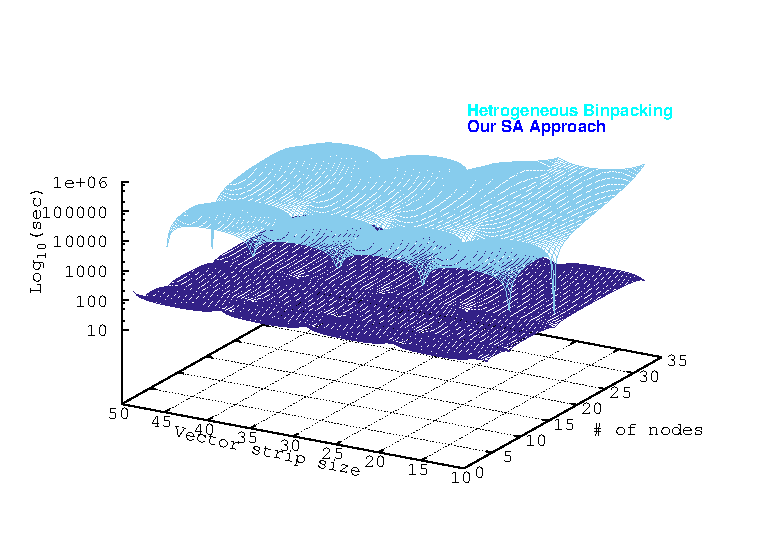
\includegraphics[angle=0, scale=0.6]{./figures/conv_hbp_surface}
%     \label{fig:conv1ho}
%   }
%   \subfigure[Gram Schmidt linear-algebra kernel]{
%     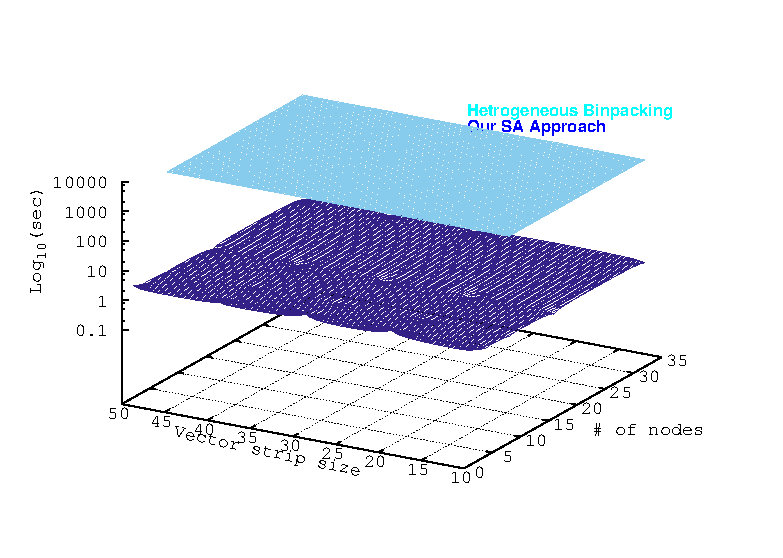
\includegraphics[angle=0, scale=0.6]{./figures/gram_hbp_surface}
%     \label{fig:gram1ho}
%   }
%   \subfigure[2 Dimensional Jacobi stencil computation]{
%     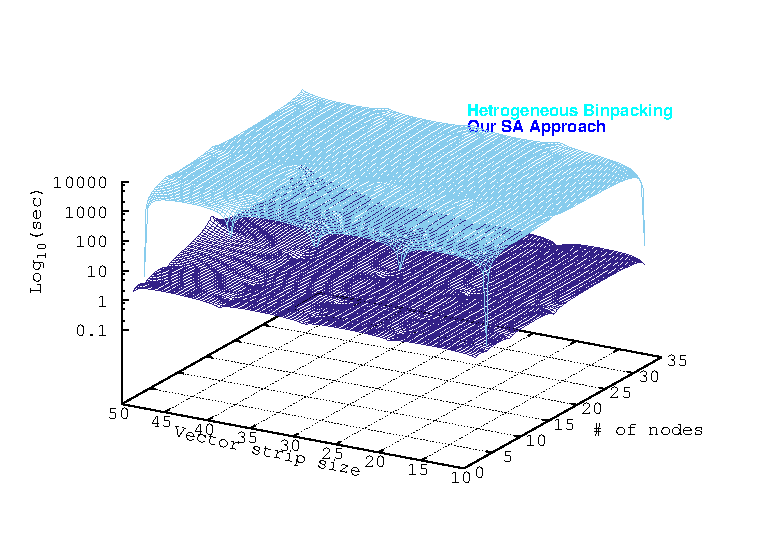
\includegraphics[angle=0, scale=0.6]{./figures/jac_hbp_surface}
%     \label{fig:jacl1ho}
%   }
%   \caption{Comparison of execution times of ``Our SA technique" and
%     ``Heterogeneous Bin Packing" (looks better in color)}
%   \label{fig:ho}
% \end{figure*}


% \subsubsection{Comparison with established SA}
% \label{sec:comp-with-establ}

% The figures showing the comparison of our approach with the established
% SA approach of~\cite{hors06} as shown in Figure~\ref{fig:stdsa}. There
% is not a single case where our SA approach is worse than the current
% established technique. The major statistics comparing the two techniques
% for Figure~\ref{fig:stdsa} are shown in Table~\ref{tab:4}.

% The reasons for this are two fold,
% \begin{itemize}
% \item We change the annealing schedule such that the search exploration is
% global initially, i.e. high temperatures, and it becomes local to the current
% best solution as temperature drops.
% \item We also get a better result because we do not permit multiple mapping
% iterations per temperature level which prevents a higher percentage of tasks
% moving to random PEs. 
% \end{itemize}

% % In all the figures and statistics presented, we ran the conventional SA and our
% % improved SA approach with a maximum time limit of 10 minutes, i.e. SA will
% % terminate after 10 minutes if it has not already found a solution it is
% % satisfied with. The experiments were performed on a quad-core dual processor
% % system with 24 gigabytes of RAM.

% \begin{figure*}[h!]
%   \centering
%   \subfigure[Binomial Option Pricing]{
%     \includegraphics[angle=0, scale=0.67]{./figures/bin_random_surface}
%     \label{fig:bin1random}
%   }
%   \subfigure[2 Dimensional Convolution]{
%     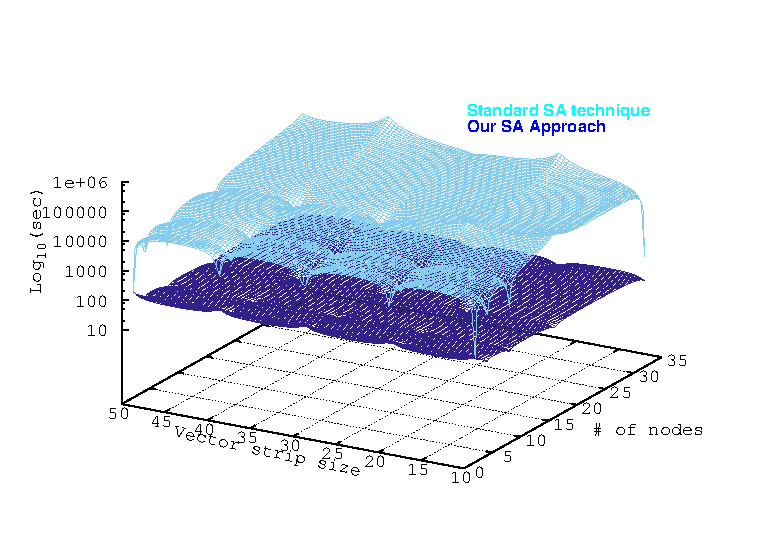
\includegraphics[angle=0, scale=0.67]{./figures/conv_random_surface}
%     \label{fig:conv1random}
%   }
%   \subfigure[Gram Schmidt linear-algebra kernel]{
%     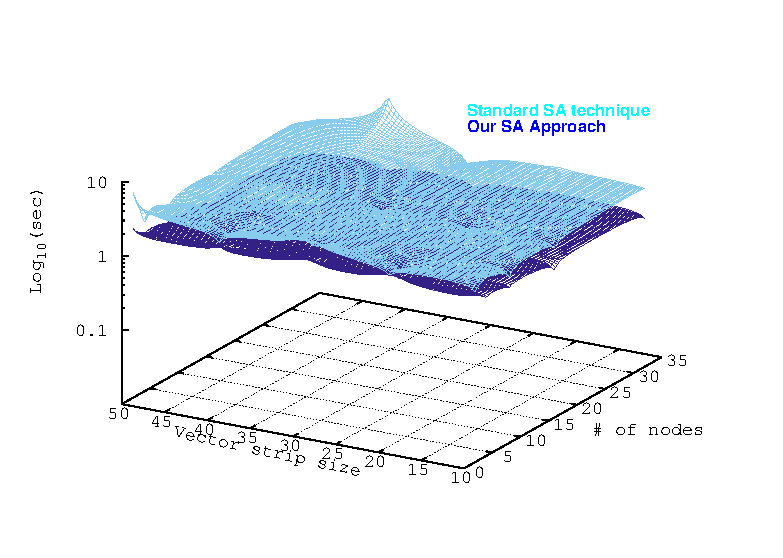
\includegraphics[angle=0, scale=0.67]{./figures/gram_random_surface}
%     \label{fig:gram1random}
%   }
%   \subfigure[2 Dimensional Seidel stencil computation]{
%     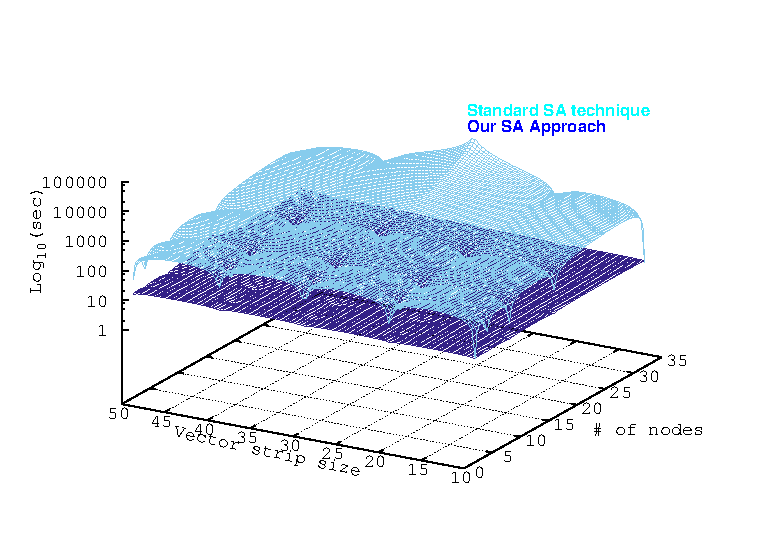
\includegraphics[angle=0, scale=0.67]{./figures/sei_random_surface}
%     \label{fig:sei1random}
%   }
%   \subfigure[2 Dimensional Jacobi stencil computation]{
%     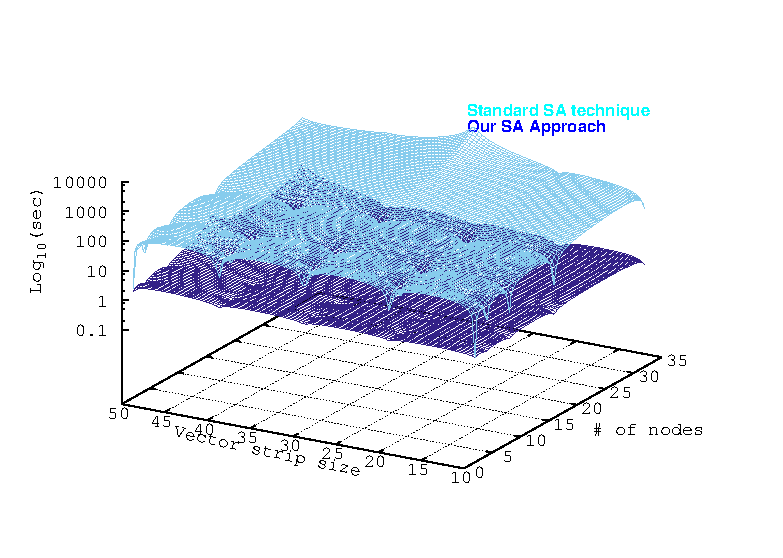
\includegraphics[angle=0, scale=0.67]{./figures/jac_random_surface}
%     \label{fig:jacl1random}
%   }
%   \caption{Comparison of application latencies: Our SA approach vs
%     standard SA approach (looks better in color)}
%   \label{fig:stdsa}
% \end{figure*}

% % \subsubsection{Effect of varying temperature}
% % \label{sec:varying-temperature}


% %%% Local Variables: 
% %%% mode: latex
% %%% TeX-master: "bare_conf"
% %%% End: 

\section{FUTURE WORK}
\label{sec:futu}

\begin{itemize}
\item One of the limiting factor in this comparison is the limited representation of the road network. We plan to extend our model by allowing edges and vertices in our road network graph to have more than one weight associated with them. In doing so, we can allow for a finer and more accurate representation of the road network which in turn allows us to partition the graph better.
\item In the modified move function, we currently move edges(the neighbour correspoding to the edge) if it has a weight which is 2$\sigma$ away from $\mu$. This is under the assumption that traffic is normally distributed across the edges. One of the improvements that we could do is to fit the distribution of traffic across edges and move edges according to this regressively found curve that fits the traffic distribution.
\end{itemize}
\section{CONCLUSION}
\label{sec:conc}

In this paper we have outlined the comparison of space and graph partitioning techniques in the context of partitioning road network graphs for simulation. We have discussed 


\section*{ACKNOWLEDGMENTS}
This work is partly funded by the IRC Enterprise Partnership Scheme in collaboration with IBM Research, Dublin, Ireland.

\appendix
\section{APPENDICES} \label{app:quadratic}
Place any appendices after the acknowledgments and label them
\textbf{A}, \textbf{B}, \textbf{C}, and so forth.


% Please don't exchange the bibliographystyle style
\bibliographystyle{wsc}
% AUTHOR: Include your bib file here
\bibliography{references}

\section*{AUTHOR BIOGRAPHIES}
\noindent {\bf ARAVIND VASUDEVAN} \\
\noindent {\bf QUENTIN BRAGARD} \\
\noindent {\bf ANTHONY VENTRESQUE} \\
\noindent {\bf DAVID GREGG}.

% \newpage
% \begin{figure*}[htb]
% {
% \centering
% First Name Last Name 1 \\
% First Name Last Name 2 \\
% \vspace{12pt}
% Institution \\
% Street Address 1 \\
% Street Address 2 \\
% City, ST Zip, COUNTRY
% \caption{Example title page heading with 2 authors from the same institution.\label{fig: 2 same}}
% }
% \end{figure*}

% \begin{figure*}[htb]
% {
% \centering
% \begin{tabular}{ccc}
% \phantom{Entries to adjust spacing - ignore} & \phantom{intermediate space} & \phantom{Entries to adjust spacing - ignore} \\
% First Name Last Name 1 & & First Name Last Name 2 \\
% \\
% Institution 1 & & Institution 2 \\
% Street Address 1 & & Street Address 1 \\
% Street Address 2 & & Street Address 2 \\
% City, ST Zip, COUNTRY & & City, ST Zip, COUNTRY
% \end{tabular}
% \caption{Example title page heading with 2 authors from different institutions.\label{fig: 2 different}}
% }
% \end{figure*}

% \begin{figure*}[htb]
% {
% \centering
% \begin{tabular}{ccc}
% \phantom{This adjusts spacing - ignore} & \phantom{This adjusts spacing - ignore} & \phantom{This adjusts spacing - ignore} \\
% First Name Last Name 1 & & First Name Last Name 2 \\
% \\
% Institution 1 & & Institution 2 \\
% Street Address Line 1 & & Street Address Line 1 \\
% Street Address Line 2 & & Street Address Line 2 \\
% City, ST Zip, COUNTRY & & City, ST Zip, COUNTRY \\
% \\
% \\
% & First Name Last Name 3 \\
% \\
% & Institution 3\\
% & Street Address 1 \\
% & Street Address 2 \\
% & City, ST Zip, COUNTRY
% \end{tabular}
% \caption{Alternate example title page heading with 3 authors from different institutions. \label{fig: 3 different}}
% }
% \end{figure*}

% \begin{figure*}[htb]
% {
% \centering
% \begin{tabular}{ccc}
% \phantom{Adjust spacing using these entries} & \phantom{intermediate space} & \phantom{Adjust spacing using these entries} \\
% First Name Last Name 1 & & First Name Last Name 2 \\
% \\
% Institution 1 & & Institution 2 \\
% Street Address Line 1 & & Street Address Line 1 \\
% Street Address Line 2 & & Street Address Line 2 \\
% City, ST Zip, COUNTRY & & City, ST Zip, COUNTRY \\
% \\ \\
% First Name Last Name 3 & & First Name Last Name 4 \\
% \\
% Institution 3 & & Institution 4 \\
% Street Address Line 1 & & Street Address Line 1 \\
% Street Address Line 2 & & Street Address Line 2 \\
% City, ST Zip, COUNTRY & & City, ST Zip, COUNTRY
% \end{tabular}
% \caption{Example title page heading with 4 authors from different institutions.\label{fig: 4 different}}
% }
% \end{figure*}

\end{document}
